\documentclass[a4paper,11pt]{article}
\usepackage[T1]{fontenc}
\usepackage[utf8]{inputenc}
\usepackage[top=1cm, bottom=1cm, left=1cm, right=1cm]{geometry}
\usepackage{listings}
\usepackage{color}
\usepackage{tikz}
\usepackage{lscape}

\tikzset{% 
  tree/.style = {
    sibling distance=15em,
    every node/.style = {shape=rectangle, rounded corners,
      draw, align=center,
      top color=white, bottom color=blue!20},
    edge from parent/.style = {draw,-latex}
  }
}

\definecolor{codegreen}{rgb}{0,0.6,0}
\definecolor{codegray}{rgb}{0.5,0.5,0.5}
\definecolor{codepurple}{rgb}{0.58,0,0.82}
\definecolor{backcolour}{rgb}{0.95,0.95,0.92}
 
\lstdefinestyle{mystyle}{
    backgroundcolor=\color{backcolour},   
    commentstyle=\color{codegreen},
    keywordstyle=\color{magenta},
    numberstyle=\tiny\color{codegray},
    stringstyle=\color{codepurple},
    basicstyle=\footnotesize,
    breakatwhitespace=false,         
    breaklines=true,                 
    captionpos=b,                    
    keepspaces=true,                 
    numbers=left,                    
    numbersep=5pt,                  
    showspaces=false,                
    showstringspaces=false,
    showtabs=false,                  
    tabsize=2
}
 
\lstset{style=mystyle}

\begin{document}
  \begin{landscape}
    \begin{figure}[h!]
      \centering
      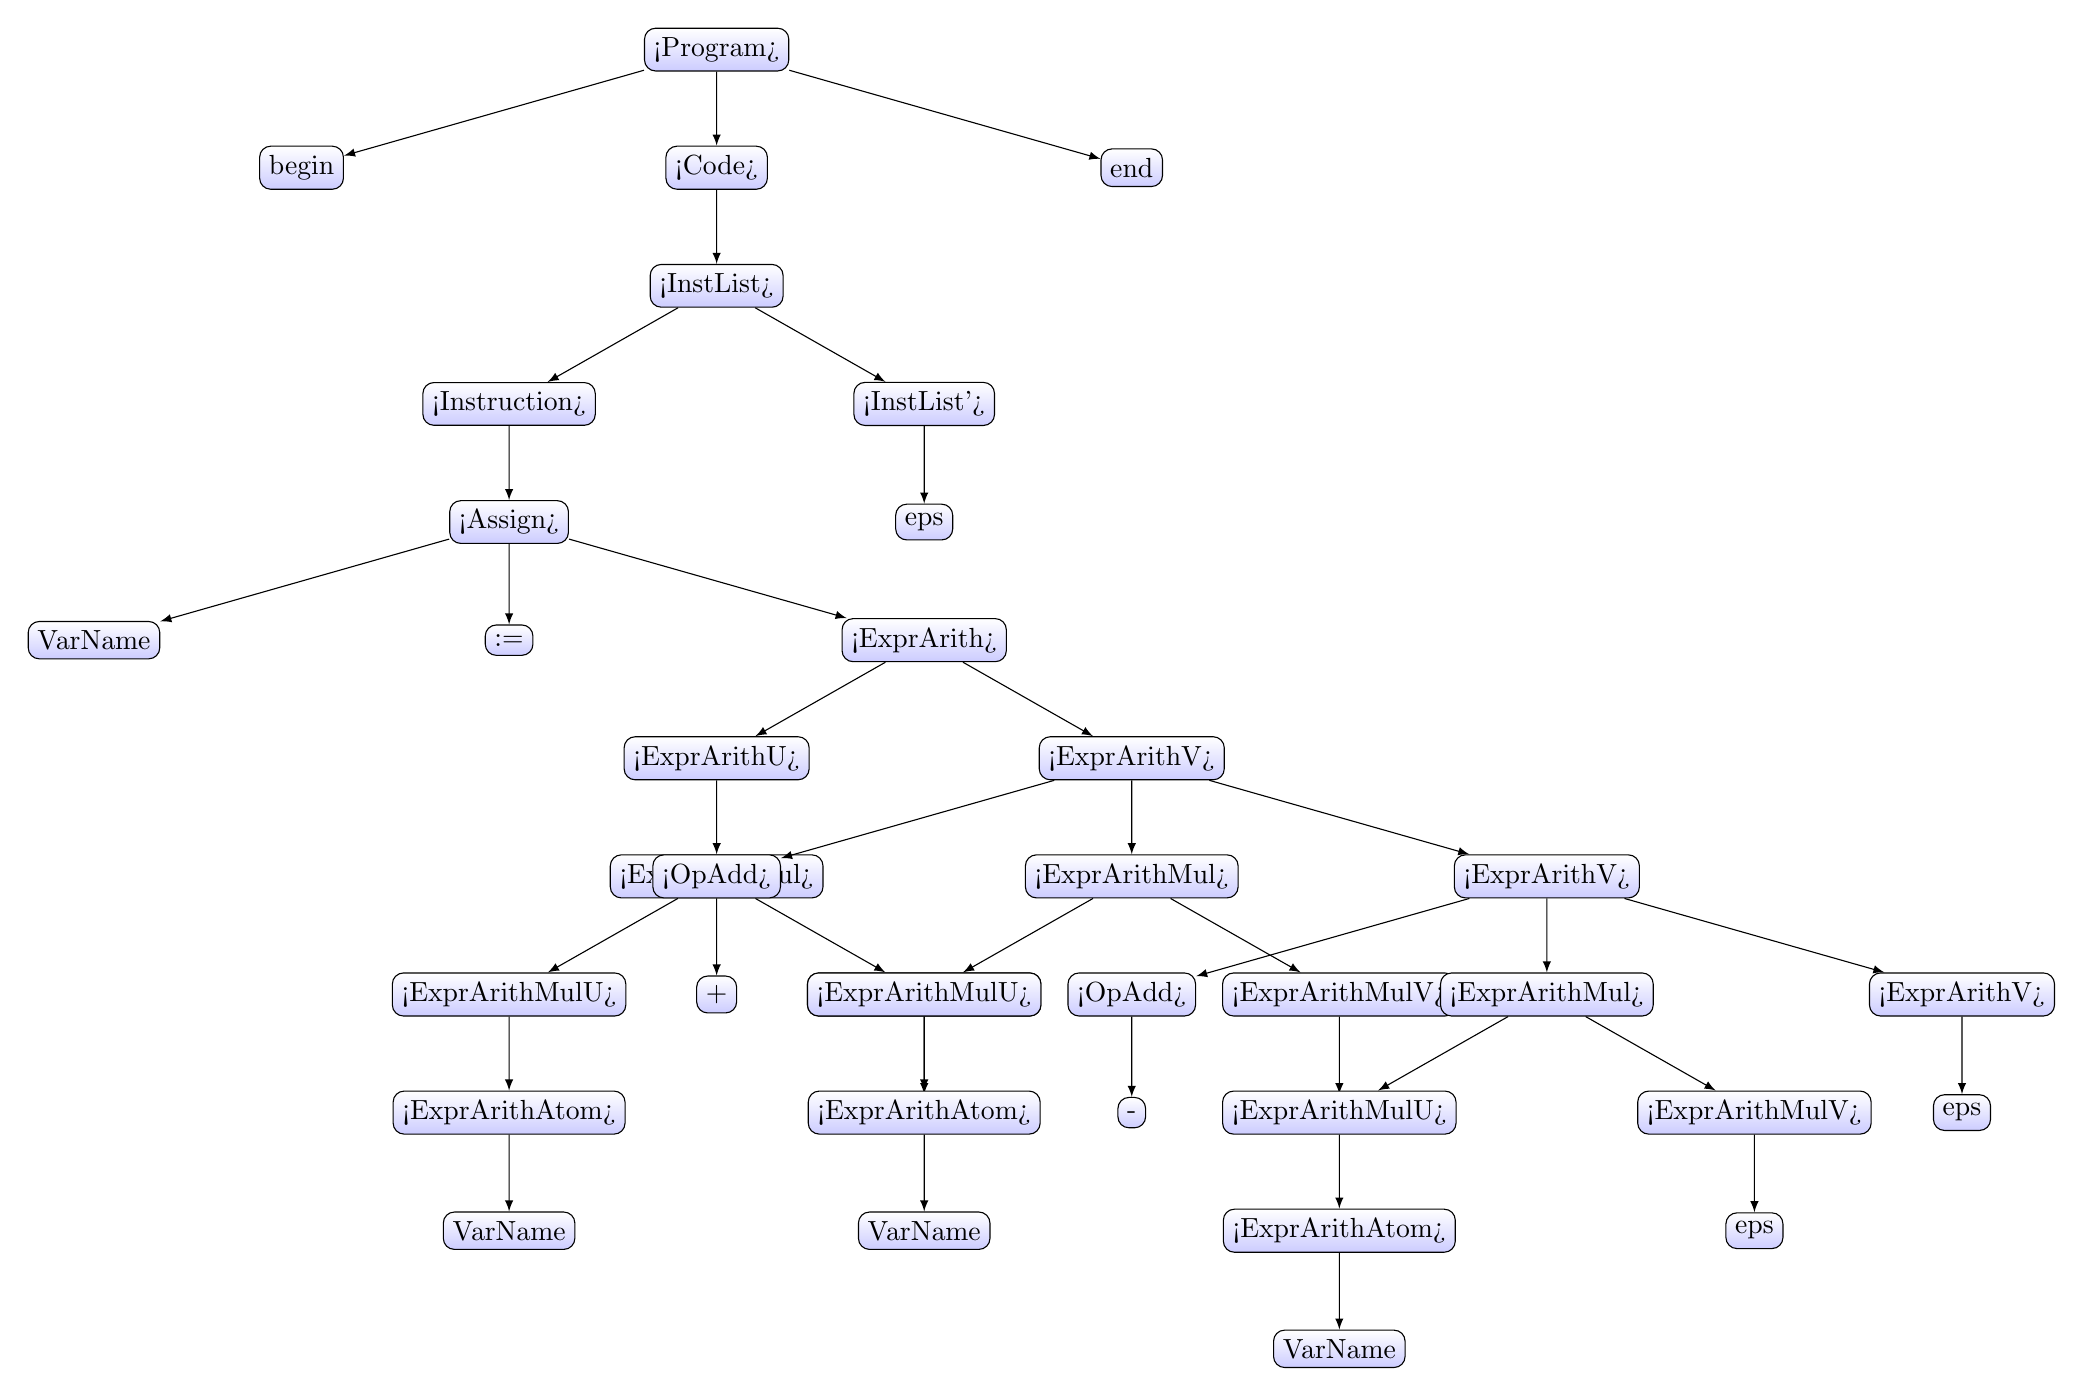
\begin{tikzpicture}[tree]
\node {<Program>}
 child {
node {begin}
}
 child {
node {<Code>}
 child {
node {<InstList>}
 child {
node {<Instruction>}
 child {
node {<Assign>}
 child {
node {VarName}
}
 child {
node {:=}
}
 child {
node {<ExprArith>}
 child {
node {<ExprArithU>}
 child {
node {<ExprArithMul>}
 child {
node {<ExprArithMulU>}
 child {
node {<ExprArithAtom>}
 child {
node {VarName}
}
}
}
 child {
node {<ExprArithMulV>}
 child {
node {eps}
}
}
}
}
 child {
node {<ExprArithV>}
 child {
node {<OpAdd>}
 child {
node {+}
}
}
 child {
node {<ExprArithMul>}
 child {
node {<ExprArithMulU>}
 child {
node {<ExprArithAtom>}
 child {
node {VarName}
}
}
}
 child {
node {<ExprArithMulV>}
 child {
node {eps}
}
}
}
 child {
node {<ExprArithV>}
 child {
node {<OpAdd>}
 child {
node {-}
}
}
 child {
node {<ExprArithMul>}
 child {
node {<ExprArithMulU>}
 child {
node {<ExprArithAtom>}
 child {
node {VarName}
}
}
}
 child {
node {<ExprArithMulV>}
 child {
node {eps}
}
}
}
 child {
node {<ExprArithV>}
 child {
node {eps}
}
}
}
}
}
}
}
 child {
node {<InstList'>}
 child {
node {eps}
}
}
}
}
 child {
node {end}
}
;      \end{tikzpicture}
    \end{figure}
  \end{landscape}
 
\end{document}

